\chapter{Metodología de la Investigación}
\section{Diseño de la investigación}
En esta sección se detallará el diseño, tipo y enfoque de la investigación, así como la población y la muestra.

\subsection{Tipo de investigación}
Se ha identificado que este estudio posee un diseño experimental con el propósito de establecer el tipo de investigación. Como lo dice \cite{bk_hernandez2014metodologia}, en la obra titulada \citetitle{bk_hernandez2014metodologia}, busca determinar la consecuencia de una razón manipulada. Específicamente, se clasifica como un diseño experimental puro debido a la utilización intencionada de variables independientes (modificadas, eliminadas o añadidas) para evaluar su influencia en la variable dependiente, que en este caso es la segmentación avanzada de características morfológicas faciales (arrugas y manchas) en imágenes de rostros faciales.

\subsection{Enfoque de la investigación}
Este estudio adoptó un enfoque cuantitativo, conforme a lo explicado por \cite{bk_hernandez2014metodologia} en su libro \citetitle{bk_hernandez2014metodologia}. Este enfoque se basa en la recopilación de datos para comprobar hipótesis mediante mediciones numéricas y análisis estadísticos, con el objetivo de identificar patrones de comportamiento y validar teorías. La metodología empleada sigue los diez pasos del proceso cuantitativo descritos por el autor, aplicados desde la formulación de la idea hasta la presentación de los resultados finales en el informe de investigación, ya que se busca desarrollar un sistema de segmentación para detectar características morfológicas de la piel facial mediante redes neuronales convolucionales (CNN) y analizar su efectividad con métricas cuantitativas, como precisión, recall, F1-score y AUC-ROC. Este enfoque permitirá evaluar el desempeño del sistema en la detección de arrugas y manchas, proporcionando resultados medibles y objetivos. 

\subsection{Población}
La población de este estudio se compone de imágenes faciales representativas de personas con diversas edades, géneros y tipos de piel. Específicamente, estas imágenes muestran características morfológicas que se asocian con arrugas y manchas faciales. Debido a la orientación del enfoque en el problemas estéticos, la población abarcaba imágenes de piel con claras imperfecciones y piel sin e incidencias asignadas. Así, el alcance de la población se determina como diverso y completo, asegurando la inclusión de imágenes que representa una amplia gama de condiciones de la piel. Finalmente, resulta esencial agregar diversidad geográfica, ya que ciertas diferencias geográficas.
\subsection{Muestra}
La muestra de la investigación comprenderá una parte de aproximadamente 5000 retratos faciales. Estas imágenes se seleccionarán mediante muestreo basado en estratos, lo que garantizará una representación uniforme en diferentes categorías de edad, identidades masculinas y femeninas y pigmentación dérmica variable La lista también tendrá imágenes con diferentes tamaños y claridad, mostrando varios tipos de arrugas y manchas, asegurándose de que el grupo muestre condiciones reales de la piel Los usaremos para enseñar, verificar y desafiar nuestro modelo de segmentación avanzada, asegurándonos de que funcione bien en la vida real con mucha variedad.

\subsection{Operacionalización de Variables}
Los detalles acerca de cómo se definen y miden las variables de estudio se presentan en la Tabla \ref{tabla:variables}.


\begin{longtable}{>{\centering\arraybackslash}m{3cm} >{\centering\arraybackslash}m{2.5cm} >{\centering\arraybackslash}m{2.5cm} >{\raggedright\arraybackslash}m{7cm}}
    \caption{Matriz de Variables Principales.}
    \label{tabla:variables}\\
    \hline
    VARIABLE & DIMENSIÓN & INDICADOR & CÁLCULO \\
    \hline
    Independiente: Imágenes de Rostros Faciales & Calidad de la Imagen & Resolución & Número de píxeles por pulgada (ppi) de la imagen, obtenido automáticamente. \\
    \cline{2-4}
     & Detalle de Rostro Facial & Características Morfológicas Faciales Identificables & Conteo de arrugas y manchas detectadas manual o automáticamente. \\
    \hline
    Dependiente: Modelo de Segmentación Avanzada de Características Morfológicas Faciales & Precisión & Diferencia de Segmentación del Modelo vs Real & $\text{Precisión} = \frac{VP}{VP + FP}$ \\ 
    \cline{2-4}
     & Índice de Sørensen–Dice & Similitud espacial & $\text{DSC} = \frac{2 \times |A \cap B|}{|A| + |B|}$ \\
    \cline{2-4}
     & Coeficiente de Jaccard & Similitud de conjunto & $\text{IoU} = \frac{|A \cap B|}{|A \cup B|}$ \\
    \cline{2-4}
     & Entropía Cruzada & Desempeño de clasificación del modelo & $\text{CE} = -\sum_{i=1}^{N} y_i \log(\hat{y}_i)$ \\
    \hline
\end{longtable}
\begin{flushleft}
	\small Fuente: Elaboración propia.
\end{flushleft}

\section{Técnicas de recolección de datos}
La recolección de imágenes de características morfológicas faciales es un paso crucial para la creación del modelo de segmentación avanzada de estas. Una de las técnicas más accesibles y efectivas para obtener estas imágenes es a través del uso de bases de datos públicas como se ve en la Figura \ref{3:fig2} y repositorios en línea. Estas fuentes ofrecen una amplia variedad de imágenes de rostros faciales, que pueden ser utilizados para modelar y crear el modelo de segmentación avanzada.

\begin{figure}[h]
	\begin{center}
		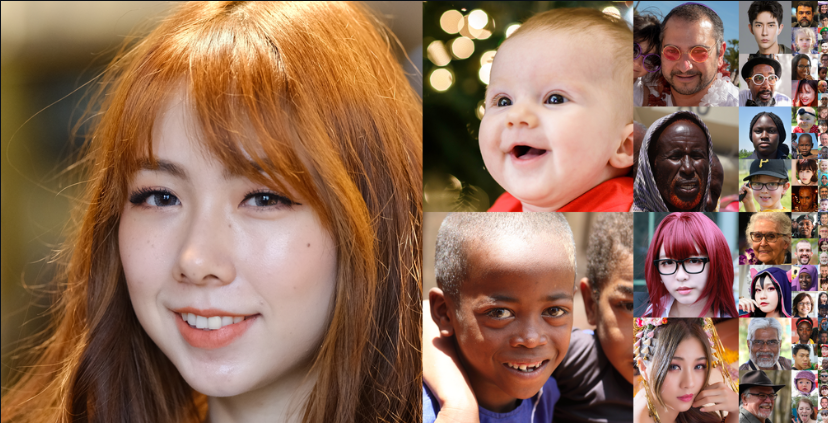
\includegraphics[width=0.5\textwidth]{3/figures/repo_github.png}
		\caption[Base de datos pública Flickr-Faces-HQ Dataset (FFHQ)]{Base de datos pública Flickr-Faces-HQ Dataset (FFHQ).\\
		Fuente: Elaboración propia}
		\label{3:fig2}
	\end{center}
\end{figure}

\begin{itemize}
    \item \textbf{Repositorios de Datasets de Imágenes Faciales}: Existen múltiples repositorios en línea dedicados específicamente a la recopilación y distribución de imágenes faciales. Plataformas como Kaggle, Papers with Code, y OpenML ofrecen conjuntos de datos etiquetados que incluyen rostros humanos con diferentes características morfológicas como arrugas, manchas, expresiones y edades. Estos datasets son fundamentales para el entrenamiento y evaluación de modelos de redes neuronales convolucionales, y suelen estar acompañados de documentación sobre su uso y licencia.
	\item \textbf{Bibliotecas Digitales y Bases de Datos Académicas}: Las bibliotecas digitales y bases de datos académicas también representan una fuente valiosa para obtener datasets faciales. En publicaciones académicas y tesis disponibles en plataformas como IEEE Xplore, SpringerLink, ScienceDirect y Google Scholar, es común encontrar referencias a datasets faciales utilizados en investigaciones previas. Estas fuentes permiten identificar conjuntos de datos validados por la comunidad científica y conocer sus aplicaciones en diferentes contextos, como el reconocimiento facial o el análisis de envejecimiento.
	\item \textbf{Plataformas de Código Abierto y Comunidades de Investigación}: Plataformas como GitHub, Hugging Face y Zenodo son ampliamente utilizadas por la comunidad investigadora para compartir datasets y modelos preentrenados. En estos repositorios, los investigadores publican conjuntos de imágenes faciales junto con scripts de preprocesamiento, anotaciones y arquitecturas de redes neuronales. Muchos de estos recursos se distribuyen bajo licencias abiertas (como CC BY o MIT).
  \end{itemize}


  %\newpage
\section{Técnicas para el procesamiento y análisis de la información}

\subsection{Metodología de implementación de la solución}

La creación de un Modelo de Segmentación Avanzada de Características Morfológicas varias fases de desarrollo, que van desde la recopilación de imágenes hasta su despliegue, como se menciona en el trabajo de \cite{yoon2023}. La imagen adquirida debe pasar por un proceso detallado posteriormente para alcanzar su etapa final. La metodología de esta investigación se muestra en la Figura \ref{3:fig3}.

\begin{figure}[H]
	\begin{center}
		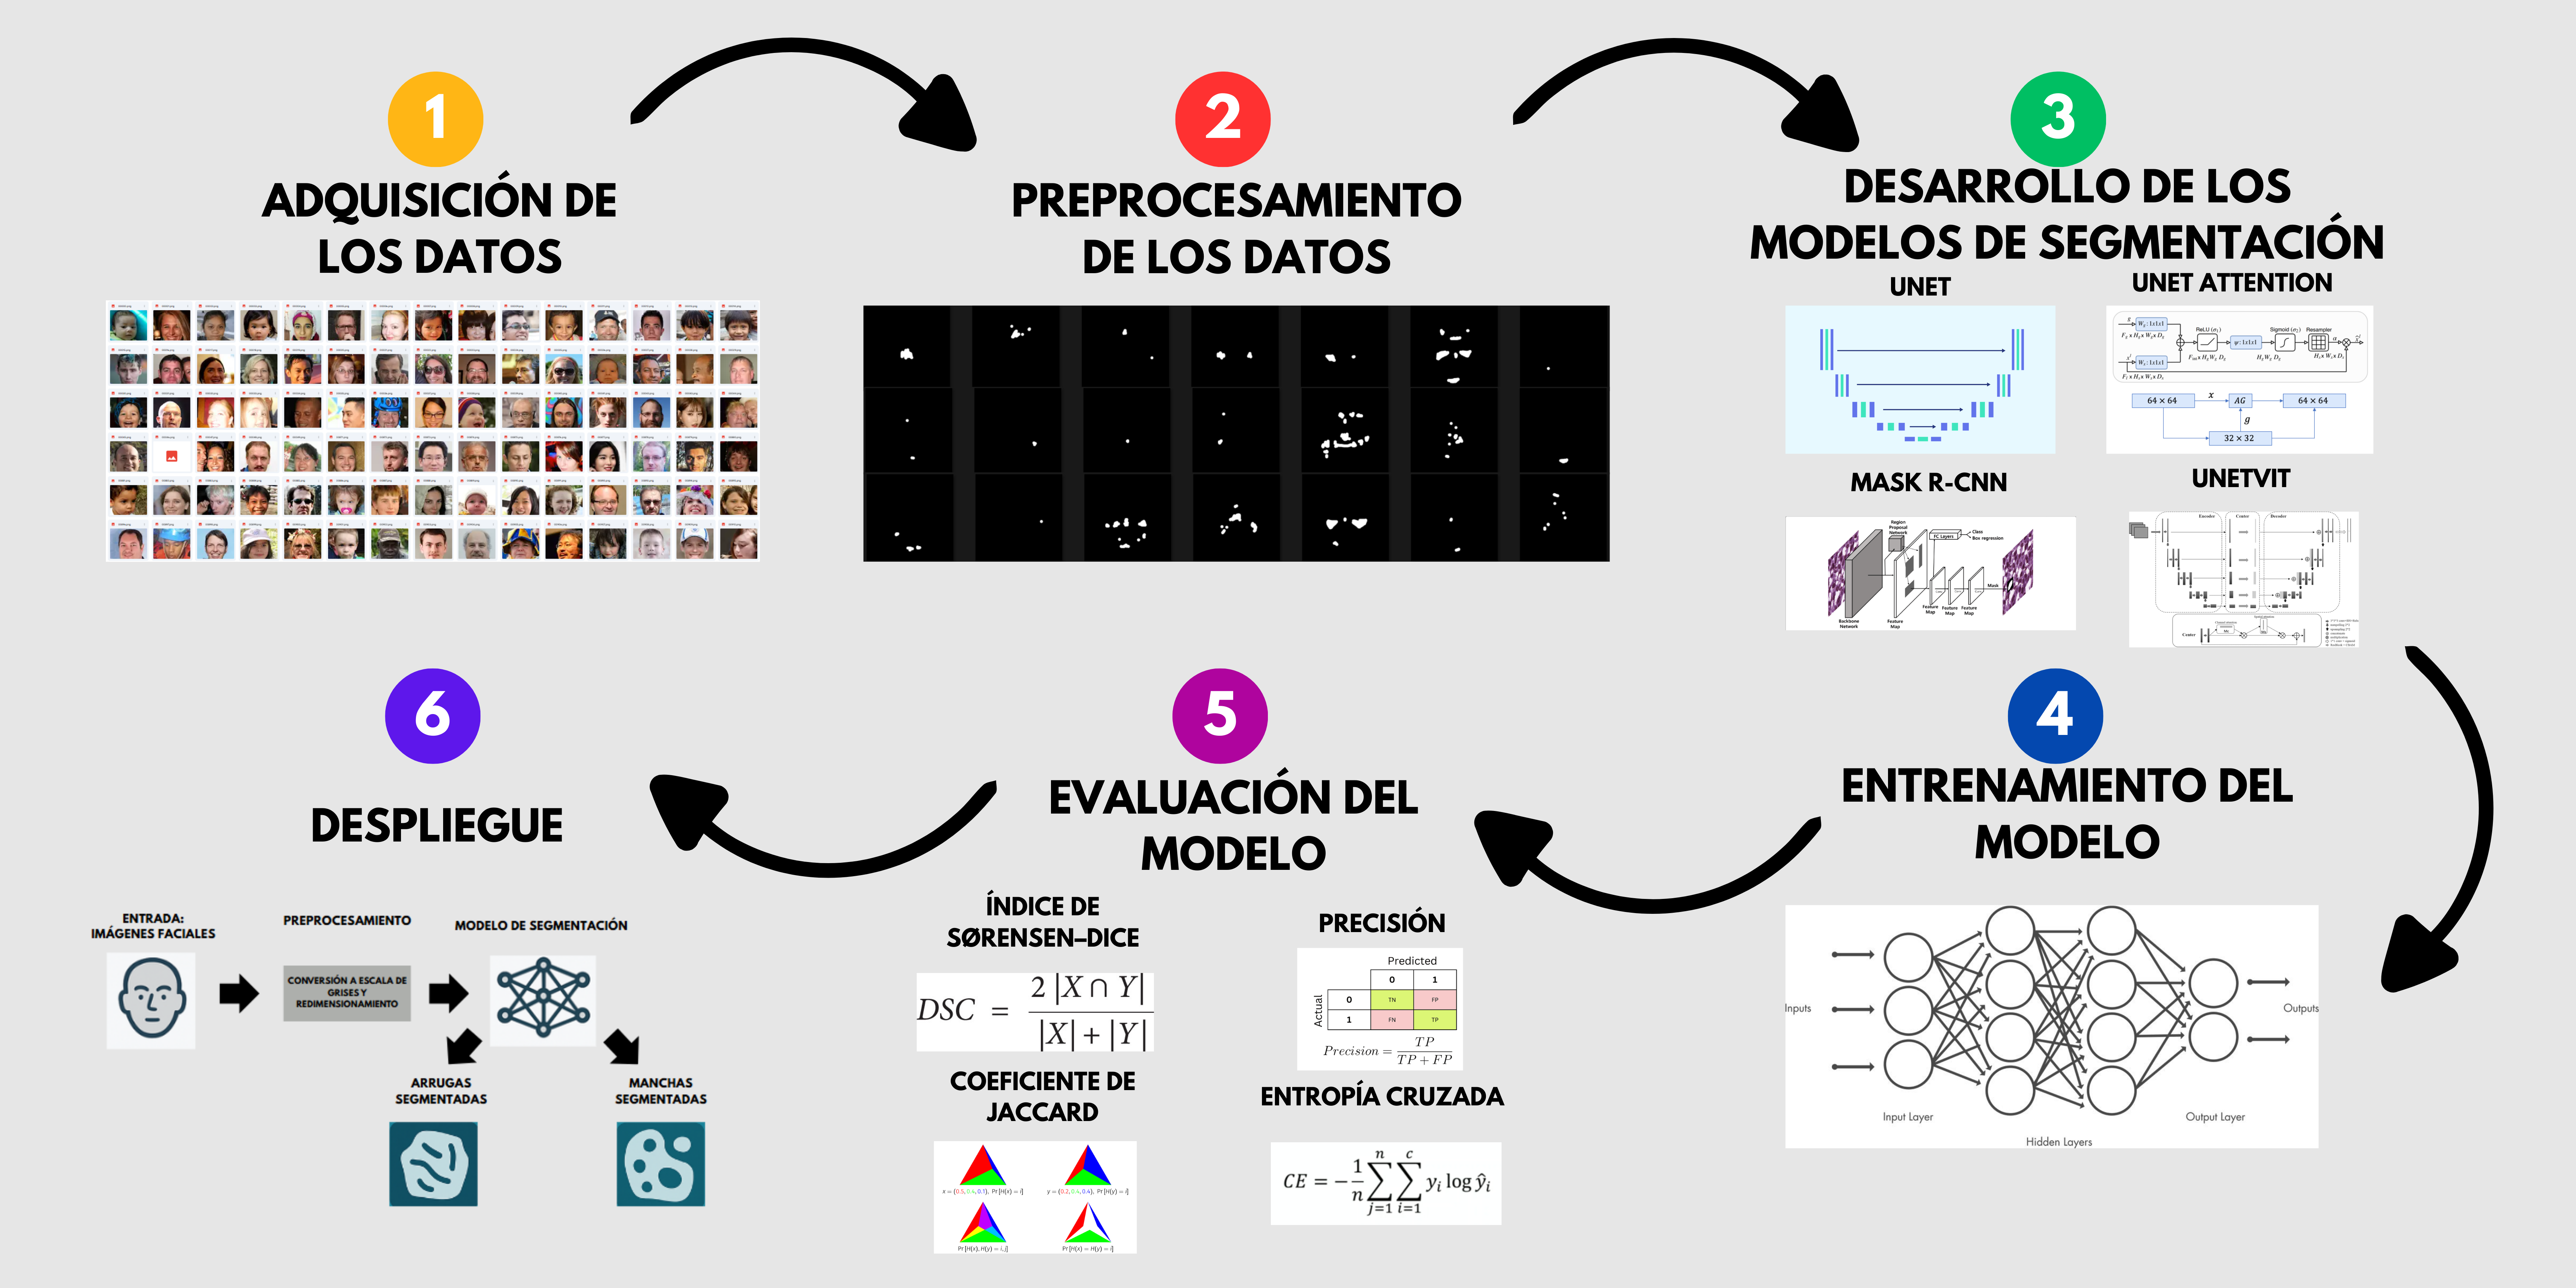
\includegraphics[width=0.8\textwidth]{3/figures/metodologia.png}
		\caption[Diagrama de Metodología de Investigación]{Diagrama de Metodología de Investigación.\\
			Fuente: Elaboración propia.}
		\label{3:fig3}
	\end{center}
\end{figure}


\subsubsection{Adquisición de los Datos}

En esta sección se describirá el procedimiento utilizado para obtener el conjunto de datos empleado en este estudio. A continuación, se presenta una tabla que resume las tareas y actividades realizadas durante esta fase de adquisición. El primer paso será la recopilación de datos. Los detalles sobre las actividades y tareas se encuentran en la Tabla \ref{tabla:actividades}.
 
 %% segunda tabla
 \begin{longtable}{>{\raggedright\arraybackslash}p{4cm} >{\raggedright\arraybackslash}p{4cm} >{\raggedright\arraybackslash}p{5cm}}
    \caption{Tabla de la Adquisición de Datos.}
    \label{tabla:actividades}\\
    \hline
    \textbf{Actividades} & \textbf{Descripción} & \textbf{Tareas}\\
    \hline
    \endfirsthead

    \multicolumn{3}{c}%
    {{\bfseries \tablename\ \thetable{} -- continuación de la página anterior}} \\
    \hline
    \textbf{Actividades} & \textbf{Descripción} & \textbf{Tareas}\\
    \hline
    \endhead

    \hline
    \multicolumn{3}{r}{{Continúa en la siguiente página}} \\
    \endfoot

    \hline
    \endlastfoot

    \textbf{Actividad 1:} Identificación de la data que contengan imágenes de rostros con características morfológicas faciales. & Identificación de la data que contengan imágenes de rostros con características morfológicas faciales relevantes para la investigación. & 
    \begin{itemize}
        \item Analizar y identificar bases de datos con rostros con características morfológicas faciales.
        \item Confirmar que la base de datos esté disponible públicamente y sea pertinente para el estudio.
        \item Descargar los datos desde el repositorio apropiado.
    \end{itemize} \\
\end{longtable}

\begin{flushleft}
    \small Fuente: Elaboración propia.
\end{flushleft}


Enseguida, se proporcionará un detalle de la actividad mencionada en la tabla anterior, junto con los resultados que se esperan obtener.
 
\textbf{Actividad 1 de “\textit{Adquisición de los Datos}”: Identificación de la data que contengan imágenes de rostros con características morfológicas faciales de proporciones similares}
\\
Esta actividad explicará la identificación de la data. Para la data, se obtendrán más de dos mil imágenes de rostros faciales de las diferentes datas encontradas en repositorios públicos. Las imágenes de rostros faciales se encuentran en la base de datos. 
 
\textbf{Entregable}: Dataset que contiene imágenes de rostros faciales con características morfológicas, tales como arrugas y manchas.
\clearpage
\newpage
\subsubsection{Preprocesamiento de los Datos}
Se realizará el preprocesamiento de las imágenes del conjunto en esta etapa. La tabla \ref{tabla:preprocesamiento} incluye las tareas y actividades necesarias para completar la etapa de preprocesamiento:
\vspace{2ex}


\begin{longtable}{>{\raggedright\arraybackslash}p{4cm} >{\raggedright\arraybackslash}p{4cm} >{\raggedright\arraybackslash}p{5cm}}
    \caption{Actividades de la fase de Preprocesamiento de Datos.}
    \label{tabla:preprocesamiento}\\
    \toprule
    \textbf{Actividades} & \textbf{Descripción} & \textbf{Tareas} \\
    \midrule
    \endfirsthead

    \toprule
    \textbf{Actividades} & \textbf{Descripción} & \textbf{Tareas} \\
    \midrule
    \endhead

    \bottomrule
    \endfoot

    \bottomrule
    \endlastfoot

    \textbf{Actividad 1:} Filtración de imágenes faciales con características morfológicas & Eliminación de imágenes con baja resolución, mala iluminación o sin las características morfológicas de interés (arrugas y manchas), para mejorar la calidad del conjunto de datos. & 
    \begin{itemize}
        \item Eliminar imágenes borrosas, sobreexpuestas o subexpuestas.
        \item Conservar solo imágenes con resolución mínima de 128×128 píxeles.
        \item Seleccionar imágenes que contengan al menos una característica morfológica visible: arrugas o manchas.
        \item Verificar que el rostro esté completamente visible y centrado en la imagen.
    \end{itemize} \\

    \textbf{Actividad 2:} Representación y normalización de las imágenes faciales & Conversión de las imágenes a formatos adecuados para su análisis por redes neuronales convolucionales. & 
    \begin{itemize}
        \item Redimensionar todas las imágenes a un tamaño uniforme.
        \item Convertir las imágenes a escala de grises o RGB, según el modelo.
        \item Normalizar los valores de píxeles entre 0 y 1.
        \item Aumentar los datos mediante técnicas como rotación, volteo, y zoom para mejorar la generalización.
    \end{itemize} \\

\end{longtable}

\begin{flushleft}
	\small Fuente: Elaboración propia.
\end{flushleft}

Enseguida, se describirá en detalle las actividades junto con el resultado esperado.

\textbf{Actividad 1 de “\textit{Preprocesamiento de los Datos}”: Filtración de imágenes faciales con características morfológicas}
\\
En la fase de preprocesamiento de datos, la actividad de Filtración se enfocará en depurar y mejorar la calidad del conjunto de datos al eliminar información irrelevante o poco confiable. Esto se logrará a través de la eliminación de datos no estándar y la conservación de aquellos que cumplen con criterios específicos de relevancia y fiabilidad. 

\textbf{Entregable}: Conjunto de datos filtrado y optimizado para su posterior análisis.

\textbf{Actividad 2 de “\textit{Preprocesamiento de los Datos}”: Representación y normalización de las imágenes faciales}
\\
Por otro lado, la actividad de Representación se encargará de convertir los datos en un formato visual o estructurado más adecuado para su análisis y comprensión. Esto implicará transformar los datos en imágenes o representaciones gráficas que faciliten su visualización y entendimiento, contribuyendo así a una mejor interpretación por parte de los usuarios finales, como podemos observar en la Figura \ref{3:fig4}.

\textbf{Entregable}: Representación visual y estructurada de cada rostro facial en un formato adecuado para su procesamiento y análisis posterior.

\begin{figure}[H]
     \begin{center}
         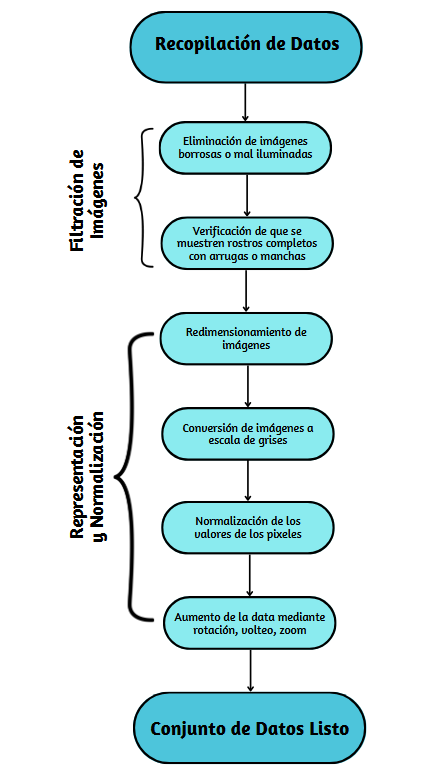
\includegraphics[width=0.6\textwidth]{3/figures/Diagrama de preprocesamiento.png}
         \caption[Diagrama Esperado de Preprocesamiento de los Datos]{Diagrama Esperado de Preprocesamiento de los Datos.\\
         Fuente: Elaboración propia}
         \label{3:fig4}
     \end{center}
 \end{figure}

\clearpage
\newpage
 \subsubsection{Desarrollo de los Modelos de Segmentación}
 El desarrollo de los modelos de segmentación de características faciales se estructurará en tres actividades clave. Estas actividades incluirán el diseño, implementación y entrenamiento de modelos basados en arquitecturas de redes neuronales profundas como U-Net, U-Net Attention, Mask R-CNN y modelos híbridos con Vision Transformer como por ejemplo Unet MiT-B0. La Tabla \ref{tabla:actividades_segmentacion} presenta el detalle de cada una.

 \vspace{2ex}
 \begingroup
 \renewcommand\arraystretch{1.2}
 \begin{longtable}{>{\raggedright\arraybackslash}p{4cm} >{\raggedright\arraybackslash}p{4cm} >{\raggedright\arraybackslash}p{5cm}}
 \caption{Actividades de la fase de Desarrollo del Modelo de Segmentación.}
 \label{tabla:actividades_segmentacion}\\
 \toprule
 \textbf{Actividades} & \textbf{Descripción} & \textbf{Tareas} \\
 \midrule
 \endfirsthead
 
 \toprule
 \textbf{Actividades} & \textbf{Descripción} & \textbf{Tareas} \\
 \midrule
 \endhead
 
 \bottomrule
 \endfoot
 
 \textbf{Actividad 1:} Diseño de la arquitectura del modelo & Selección conceptual y estructural de modelos apropiados para la segmentación de características morfológicas faciales. &
 \begin{itemize}
     \item Análisis de U-Net para segmentación precisa de áreas pequeñas como arrugas y manchas.
     \item Evaluación del potencial de Mask R-CNN para representar características profundas y complejas.
     \item Consideración de arquitecturas híbridas que integren Unet con Vision Transformer (Unet MiT-B0).
 \end{itemize} \\
 
 \textbf{Actividad 2:} Definición de componentes del modelo & Establecimiento de las partes esenciales del modelo para la segmentación de imágenes faciales. &
 \begin{itemize}
     \item Diseño de capas convolucionales, de codificación y decodificación.
     \item Propuesta de bloques residuales y mecanismos de atención en modelos híbridos.
     \item Configuración de dimensiones de entrada y salida adaptadas a imágenes faciales.
 \end{itemize} \\
 
 \end{longtable}
 \endgroup

 Enseguida, se proporcionará en la Figura \ref{3:fig5} el diagrama de cada actividad, y a su vez un detalle de la actividad junto con el entregable correspondiente que se espera obtener.
 
 \textbf{Actividad 1 de “\textit{Desarrollo de los Modelos de Segmentación}”: Diseño de la arquitectura del modelo}
 \\
 Durante esta etapa se definirá la estructura general de las redes neuronales que se utilizarán para la segmentación de características morfológicas faciales. El objetivo será seleccionar arquitecturas que sean adecuadas para extraer información precisa de regiones faciales como arrugas o manchas.
 Entre las arquitecturas consideradas se encontrarán U-Net, que destaca por su capacidad de segmentación precisa gracias a su estructura simétrica y sus conexiones de salto entre el codificador y el decodificador. También se evaluará el uso de Mask R-CNN, una arquitectura que incorpora bloques residuales para mejorar el aprendizaje en redes profundas, especialmente útil para capturar texturas complejas. Asimismo, se contemplará la exploración de modelos híbridos que combinan Unet con Vision Transformer (Unet MiT-B0), lo cual permitirá captar patrones sutiles mediante mecanismos de atención.
 
 \textbf{Entregable}: Selección de la arquitectura óptima para el modelo de segmentación facial, justificada técnicamente.

 \textbf{Actividad 2 de “\textit{Desarrollo de los Modelos de Segmentación}”: Definición de componentes del modelo}
 \\
Esta actividad consistirá en establecer los elementos esenciales que conformarán las redes previamente seleccionadas. Se determinará la cantidad de capas, el tipo de operaciones dentro de cada módulo y la forma en que se conectan entre sí, en función de las necesidades de segmentación facial.

En U-Net, por ejemplo, se definirá cuántas capas de codificación y decodificación se utilizarán, así como las conexiones que transmitirán información detallada entre estas. En Mask R-CNN, se especificará el número de bloques residuales y la profundidad de la red, asegurando que se mantenga la eficiencia del aprendizaje sin perder información relevante. En los modelos híbridos como Unet MiT-B0, se determinará cómo integrar los módulos de atención con las capas convolucionales, de forma que se mantenga un flujo eficiente de características entre ambos entornos.

 \textbf{Entregable}: Especificación detallada de los componentes y estructura interna de cada arquitectura seleccionada.

 
 \begin{figure}[H]
    \begin{center}
        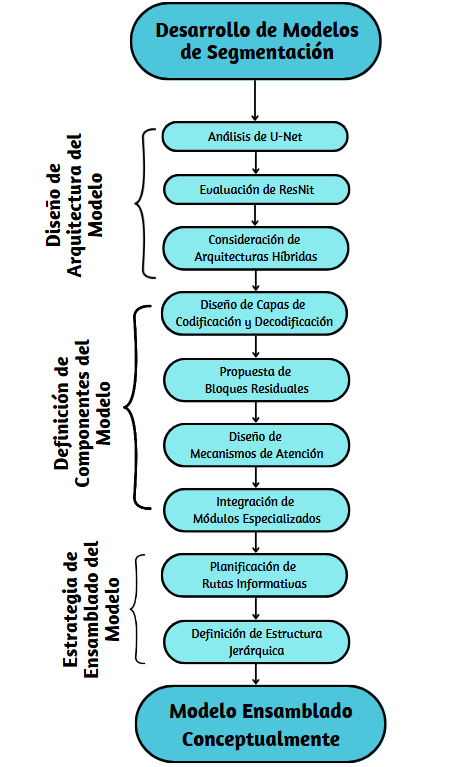
\includegraphics[width=0.6\textwidth]{3/figures/Diagrama de Desarrollo.png}
        \caption[Diagrama Esperado del Desarrollo de los Modelos de Segmentación]{Diagrama Esperado del Desarrollo de los Modelos de Segmentación.\\
        Fuente: Elaboración propia}
        \label{3:fig5}
    \end{center}
\end{figure}
\clearpage
\newpage
\subsubsection{Entrenamiento del Modelo}
Al concluir la etapa de Desarrollo de Modelos de Segmentación, se continuará con el Entrenamiento, en la Tabla \ref{tabla:entrenamiento_modelo} fue diseñada siguiendo las actividades.

\vspace{2ex}
\begingroup
\renewcommand\arraystretch{1.2}
\begin{longtable}{>{\raggedright\arraybackslash}p{4cm} >{\raggedright\arraybackslash}p{6cm} >{\raggedright\arraybackslash}p{6cm}}
\caption{Actividades de la fase de Entrenamiento del Modelo.}
\label{tabla:entrenamiento_modelo}\\
\toprule
\centering\textbf{Actividades} & \centering\textbf{Descripción} & \centering\textbf{Tareas} \tabularnewline
\midrule
\endfirsthead

\bottomrule
\endfoot

\textbf{Actividad 1:} Configuración del entorno de entrenamiento &
Preparación del entorno computacional y los recursos necesarios para el entrenamiento del modelo. &
\begin{itemize}
    \item Selección del framework PyTorch.
    \item Habilitación del uso de GPU para acelerar el entrenamiento.
    \item Establecimiento de rutas de acceso a los datos y modelos.
\end{itemize} \\[2ex]

\textbf{Acitividad 2:} Aplicación de técnicas de optimización &
Utilización de métodos que permitan una mejora progresiva del modelo a lo largo de las épocas de entrenamiento. &
\begin{itemize}
    \item Configuración del optimizador Adam para minimizar la función de pérdida.
    \item Ajuste de tasa de aprendizaje, tamaño de batch y número de épocas.
    \item Monitorización de la evolución del loss y métricas de precisión.
\end{itemize} \\[2ex]

\textbf{Actividad 3:} Validación cruzada del rendimiento &
Evaluación del desempeño del modelo utilizando múltiples divisiones del conjunto de datos. &
\begin{itemize}
    \item División del dataset en k pliegues para pruebas y entrenamiento.
    \item Entrenamiento del modelo en diferentes subconjuntos.
    \item Análisis del promedio de métricas obtenidas para garantizar estabilidad.
\end{itemize} \\

\end{longtable}
\endgroup



 Enseguida, se proporcionará un detalle de la actividad junto con el entregable correspondiente que se espera obtener.
 
 \textbf{Actividad 1 de “\textit{Entrenamiento del modelo}”: Configuración del entorno de entrenamiento}
 \\
 Durante esta etapa se preparará el entorno computacional necesario para llevar a cabo el entrenamiento del modelo de segmentación facial. Esto implicará elegir el framework de desarrollo adecuado, como PyTorch, que permitirá implementar arquitecturas de redes neuronales de manera eficiente. Además, se habilitará el uso de aceleradores de hardware, como GPU, que reducirán considerablemente el tiempo de entrenamiento. También se configurarán las rutas para el acceso a los datos de entrada y se definirán los parámetros básicos que utilizará el entorno de ejecución.

 \textbf{Entregable}: Entorno de entrenamiento configurado y funcional, listo para ejecutar los modelos definidos.

 \textbf{Actividad 2 de “\textit{Entrenamiento del modelo}”: Aplicación de técnicas de optimización}
 \\
 En esta fase se aplicarán técnicas diseñadas para mejorar el aprendizaje del modelo durante el entrenamiento. Se implementará el optimizador Adam, ampliamente utilizado por su capacidad de ajustar dinámicamente los parámetros de la red, favoreciendo una convergencia más rápida y estable. Se determinarán parámetros críticos como la tasa de aprendizaje, el tamaño del lote (batch size) y el número total de épocas, adaptándolos al comportamiento del modelo y la complejidad del conjunto de datos. Además, se monitorearán continuamente la función de pérdida (loss) y las métricas de precisión para evaluar el progreso del modelo.

 \textbf{Entregable}: Modelo entrenado con parámetros de optimización ajustados, y registro de métricas de desempeño durante las épocas.

 \textbf{Actividad 3 de “\textit{Entrenamiento del modelo}”: Validación cruzada del rendimiento}
 \\
 El objetivo de esta actividad será evaluar de manera robusta el rendimiento del modelo mediante la técnica de validación cruzada. Se dividirá el conjunto de datos en k pliegues, permitiendo entrenar y validar el modelo en diferentes combinaciones de subconjuntos. Esta estrategia ayudará a prevenir el sobreajuste (overfitting) y asegurará que el desempeño del modelo no dependa exclusivamente de una sola partición del dataset. Finalmente, se analizará el promedio de métricas obtenidas en cada iteración para validar la estabilidad y generalización del modelo.

 \textbf{Entregable}: Reporte de resultados de validación cruzada con métricas promedio y análisis de estabilidad del modelo.
\clearpage
\newpage
\subsubsection{Evaluación del Modelo}
En esta etapa, se llevará a cabo la evaluacion de los prototipos elaborados en este trabajo, en la seccion 3.3.2 se está empleando las métricas de clasificación seleccionadas y detalladas. Se ofrece un analisis pormenorizado de las actividades y tareas ejecutadas en esta fase en la Tabla \ref{tabla:evaluacion_modelo}.

\vspace{2ex}
 \begingroup
 \renewcommand\arraystretch{1.2}
 \begin{longtable}{>{\raggedright\arraybackslash}p{4cm} >{\raggedright\arraybackslash}p{4cm} >{\raggedright\arraybackslash}p{5cm}}
 \caption{Actividades de la fase de Evaluación del Modelo.}
 \label{tabla:evaluacion_modelo}\\
 \toprule
 \textbf{Actividades} & \textbf{Descripción} & \textbf{Tareas} \\
 \midrule
 \endfirsthead
 
 \toprule
 \textbf{Actividades} & \textbf{Descripción} & \textbf{Tareas} \\
 \midrule
 \endhead
 
 \bottomrule
 \endfoot
 
 \textbf{Actividad 1:} Preparación de Datos de Validación & Seleccionar y preparar un conjunto de datos de validación representativo. & 
 \begin{itemize}
     \item Elección de imágenes que no hayan sido empleados en el proceso de entrenamiento.
     \item Preprocesamiento de imágenes.
 \end{itemize} \\
 
 \textbf{Actividad 2:} Definición de Métricas de Evaluación & Definir métricas cuantitativas para evaluar al modelo de segmentación. & 
 \begin{itemize}
     \item Identificación de métricas adecuadas.
     \item Implementación de funciones para calcular estas métricas.
 \end{itemize} \\
 
 \textbf{Actividad 3:} Evaluación del Modelo & Evaluar el modelo entrenado en el conjunto de datos de validación para obtener una línea base. & 
 \begin{itemize}
     \item Eficiencia del modelo de segmentación en el conjunto de validación.
     \item Cálculo de métricas de evaluación.
 \end{itemize} \\
 
 \end{longtable}
 \endgroup

 Enseguida, se proporcionará un detalle de la actividad junto con el entregable correspondiente que se espera obtener.


 \textbf{Actividad 1 de “\textit{Evaluación del modelo}”: Preparación de Datos de Validación}
 \\
 La preparación de los datos de validación desempeñará un papel crucial en la evaluación de la efectividad del modelo en datos no previamente vistos. Esta tarea implicará seleccionar un subconjunto representativo del conjunto de datos que no se haya utilizado durante el entrenamiento del modelo. La selección deberá tener en cuenta la diversidad en las imágenes y sus configuraciones para garantizar que el modelo pueda generalizar correctamente a diferentes escenarios.
 
 \textbf{Entregable}: Un conjunto de datos listo para su uso en la evaluación del modelo, que incluye imágenes preprocesadas y listas para ser utilizadas en el análisis.
 
 \textbf{Actividad 2 de “\textit{Evaluación del modelo}”: Definición de Métricas de Evaluación}
 \\
 Para la evaluación del rendimiento del modelo de manera cuantitativa, será esencial definir métricas claras. Estas métricas proporcionarán una base objetiva para comparar el rendimiento del modelo en diferentes escenarios y con otros enfoques existentes.
 
 \textbf{Entregable}: Un documento detallado que describe cada métrica y proporciona el código o las funciones necesarias para calcularlas.
 
 \textbf{Actividad 3 de “\textit{Evaluación del modelo}”: Evaluación del Modelo}
 \\
 La evaluación del modelo involucrará el uso del conjunto de datos de validación para establecer un punto de referencia sobre su rendimiento. Esta evaluación será esencial para comprender el comportamiento del modelo en situaciones no previamente vistas durante el entrenamiento y para identificar posibles áreas de mejora.
 
 \textbf{Entregable}: Un informe que presenta los resultados de la evaluación inicial, incluyendo las métricas de rendimiento calculadas y cualquier observación relevante sobre el comportamiento del modelo.
 \clearpage
\newpage
\subsubsection{Despliegue}
Al concluir la metodología empleada, se procederá a implementar el modelo propuesto luego de finalizar su entrenamiento y evaluación correspondiente. Los pasos y tareas realizados en esta fase se encuentran detallados en la Tabla \ref{tabla:despliegue}.

\vspace{2ex}
 \begingroup
 \renewcommand\arraystretch{1.2}
 \begin{longtable}{>{\raggedright\arraybackslash}p{4cm} >{\raggedright\arraybackslash}p{4cm} >{\raggedright\arraybackslash}p{5cm}}
 \caption{Actividades de la fase de Despliegue.}
 \label{tabla:despliegue}\\
 \toprule
 \textbf{Actividades} & \textbf{Descripción} & \textbf{Tareas} \\
 \midrule
 \endfirsthead
 
 \toprule
 \textbf{Actividades} & \textbf{Descripción} & \textbf{Tareas} \\
 \midrule
 \endhead
 
 \bottomrule
 \endfoot
 
 \textbf{Actividad 1:} Preparación del Entorno de Despliegue & Configurar el entorno necesario para desplegar el modelo en producción. & 
    \begin{itemize}
        \item Selección de infraestructura.
        \item Configuración del entorno de hardware y software.
        \item Pruebas iniciales.
    \end{itemize} \\
 
 \textbf{Actividad 2:} Despliegue del Modelo en Producción & Implementar el modelo en el entorno de producción para su uso real. & 
 \begin{itemize}
     \item Implementación del modelo en producción.
     \item Configuración de parámetros en tiempo de ejecución.
     \item Monitoreo inicial del desempeño.
 \end{itemize} \\
 \end{longtable}
 \endgroup

 Enseguida, se proporcionará un detalle de la actividad junto con el entregable correspondiente que se espera obtener.

\textbf{Actividad 1 de “\textit{Despliegue del modelo}”: Preparación del Entorno de Despliegue}
\\
La preparación del entorno de despliegue será una etapa fundamental para asegurar que el modelo de segmentación, por lo que se hizo el diseño del prototipo como se ve en la Figura \ref{3:fig6} pueda ser ejecutado eficientemente en producción. Este proceso implicará la selección y configuración de la infraestructura necesaria, incluyendo tanto hardware como software, y la realización de pruebas iniciales para confirmar que todo funciona correctamente antes del despliegue completo.

\textbf{Entregable}: Un entorno completamente preparado, con todos los componentes necesarios instalados y configurados, listo para el despliegue del modelo.

\textbf{Actividad 2 de “\textit{Despliegue del modelo}”: Despliegue del Modelo en Producción}
\\
El despliegue del modelo en producción será el paso en el que el modelo de segmentación se pone en funcionamiento en el entorno de producción. Este proceso incluirá la implementación del modelo, la configuración de parámetros necesarios para su ejecución en tiempo real, y el monitoreo inicial para asegurar que el modelo funciona correctamente en condiciones reales.

\textbf{Entregable}: El modelo está completamente implementado y operando en el entorno de producción, con los parámetros ajustados y el desempeño monitoreado para asegurar su correcto funcionamiento.

\begin{figure}[h]
    \begin{center}
        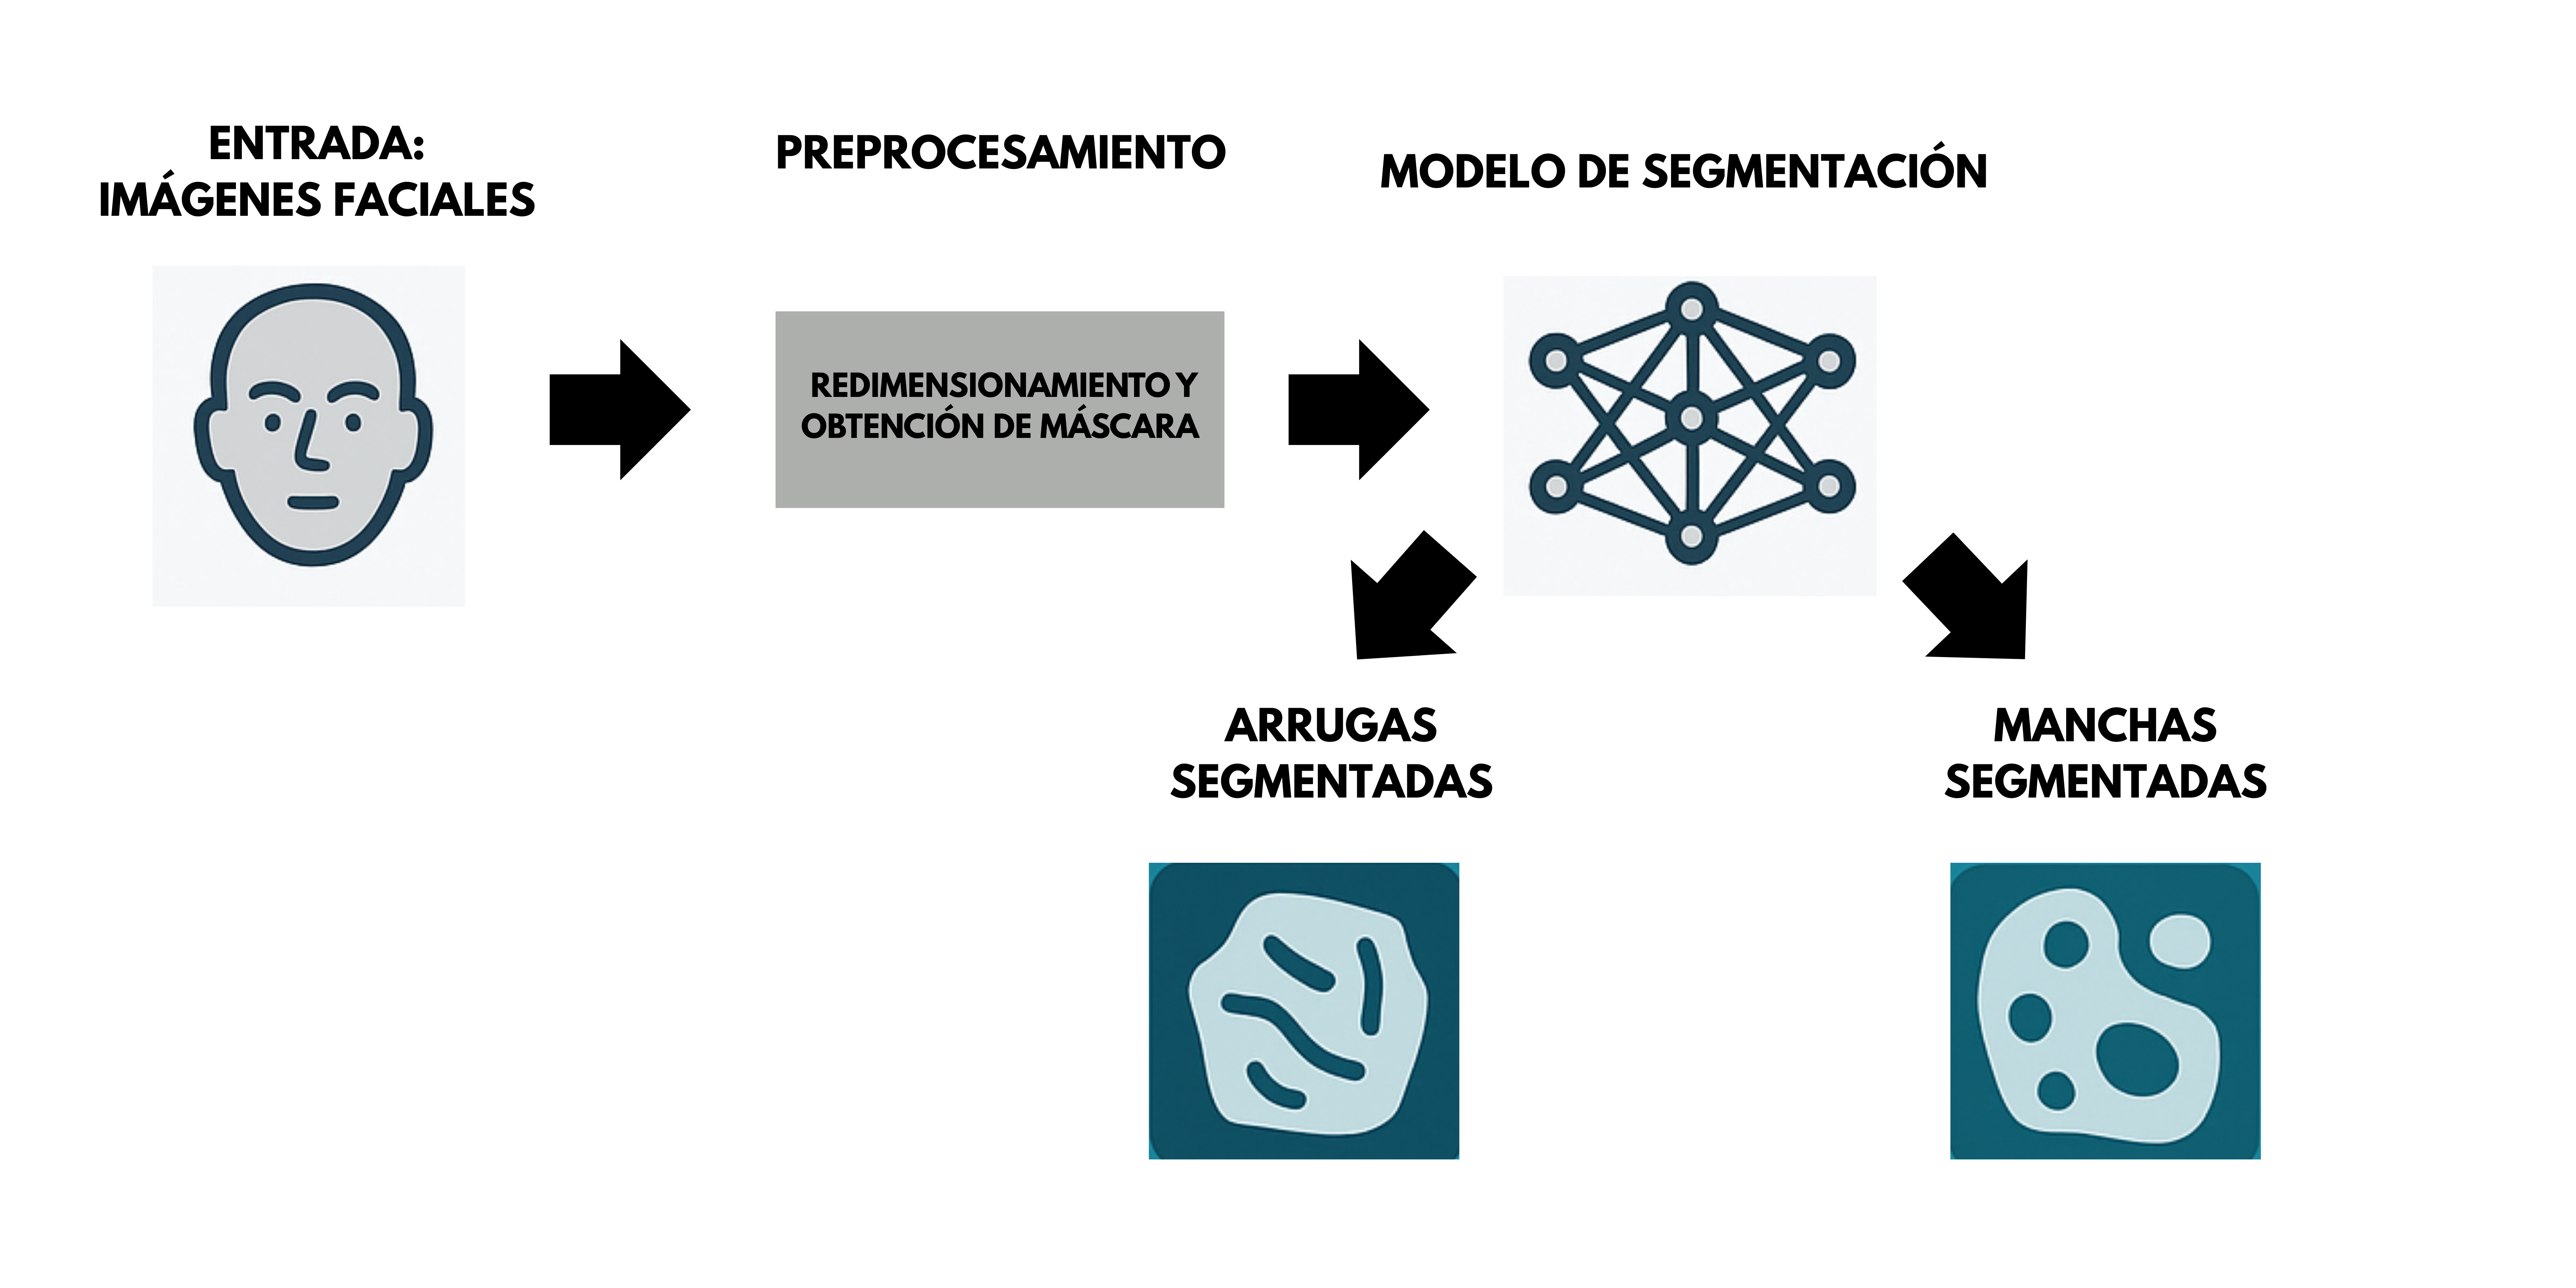
\includegraphics[width=1\textwidth]{3/figures/Prototipo de Despliegue.png}
        \caption[Proceso de operacion del prototipo del sistema]{Proceso de operacion del prototipo del sistema.\\
        Fuente: Elaboración propia}
        \label{3:fig6}
    \end{center}
\end{figure}

\section{Metodología para la Medición de Resultados de la Implementación}

Diversas métricas se emplearán para evaluar el desempeño de un modelo, en los datos de la Matriz de Confusión, sirviendo como herramientas de evaluación fundamentadas. A continuación, se describe su significado y sus componentes.

\begin{itemize}
\item \textbf{Matriz de confusión}: Tabla de dimensiones que sintetiza la precisión de predicciones generadas por un protitopo de categorización. La matriz muestra la relación entre las etiquetas predichas por el modelo y las etiquetas reales de los datos. Uno de los ejes de la matriz representa las etiquetas predichas, mientras que el otro muestra las etiquetas reales, con N representando el número total de clases. Su propósito primario es analizar la eficacia de un modelo de Aprendizaje Automático Supervisado en conjuntos de datos de prueba, donde las etiquetas reales son desconocidas. El término <<matriz de confusión>> se origina porque ayuda a identificar dónde el sistema confunde entre dos clases (Big Data, 2019) en la Figura \ref{3:fig7}, se puede encontrar una representación visual de la matriz de confusión.
\begin{figure}[H]
	\centering
	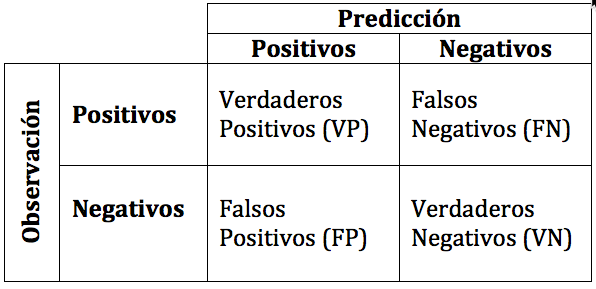
\includegraphics[width=0.75\textwidth]{3/figures/matriz_confusion.png}
	\caption[Matriz de Confusión]{Matriz de Confusión.\\ Fuente: \cite{izco2018bdc}. \citetitle{izco2018bdc}.}
	\label{3:fig7}
\end{figure}
\end{itemize}

\begin{itemize}
    \item \textbf{Verdaderos Positivos}: Se denomina verdadero positivo cuando el modelo realiza una predicción precisa de la clase positiva.
    \item \textbf{Verdaderos Negativos}: Se trata de un verdadero negativo cuando el modelo realiza una predicción correcta de la clase negativa.
    \item \textbf{Falsos Positivos}: Ocurre un falso positivo cuando el modelo hace una predicción incorrecta de la clase positiva. 
    \item \textbf{Falsos Negativos}: Ocurre un falso negativo cuando el modelo hace una predicción incorrecta de la clase negativa. 
    \end{itemize}

Después de explicar los conceptos anteriores, se obtienen diferentes métricas, de las cuales solo se utilizará la precisión métrica según lo referenciado en los documentos anteriores:

\textbf{Precisión}: evalúa la fracción de elementos detectados adecuadamente como positivos entre todos los elementos identificados como positivos. Su cálculo se basa en la siguiente expresión.
        \begin{equation}\label{eq:precision}
            \phantomsection
            \text{Precisión}=\frac{V.P.}{V.P.+F.P.}
            \end{equation}
        \myequations{Fórmula para la precisión}
        
        La pregunta que responde esta métrica es: ¿Cuál es la proporción de segmentaciones positivas que son precisas?


Además, se tomará otras métricas para evaluar el rendimiento del modelo de segmentación, las cuales se explicarán a continuación:

\textbf{Índice de Sørensen–Dice (Dice Similarity Coefficient - DSC)}
El índice de Sørensen-Dice es una medida estadística utilizada para evaluar la similitud entre dos muestras. En el contexto de segmentación de imágenes, cuantifica la superposición entre la segmentación predicha y la verdadera (ground truth). \parencite{taha2015metrics}
        
Se define como:
        
\begin{equation}
    \text{DSC} = \frac{2 \times |A \cap B|}{|A| + |B|}
\end{equation}
\myequations{Fórmula del Índice de Sørensen–Dice (DSC)}

\noindent Donde:
\begin{itemize}
    \item $|A|$ representa el número de píxeles predichos como positivos por el modelo.
    \item $|B|$ representa el número de píxeles verdaderamente positivos (segmentación real).
    \item $|A \cap B|$ es el número de píxeles correctamente clasificados como positivos (verdaderos positivos).
\end{itemize}

\noindent El Índice de Sørensen–Dice mide la superposición entre la predicción y la verdad real, con un rango de valores entre $0$ (sin coincidencia) y $1$ (coincidencia perfecta).
     

\textbf{Coeficiente de Jaccard (Índice de Intersección sobre Unión - IoU)}
El Coeficiente de Jaccard o IoU (Intersection over Union) mide la proporción de la intersección entre el área segmentada correctamente y la unión de todas las áreas predichas y reales. Es una de las métricas más comunes en segmentación de imágenes. \parencite{reinke2021common}
        
\begin{equation}
    \text{IoU} = \frac{|A \cap B|}{|A \cup B|}
\end{equation}
\myequations{Fórmula del Coeficiente de Jaccard (Intersection over Union)}

\noindent Donde:
\begin{itemize}
    \item $|A|$ es el conjunto de píxeles positivos predichos.
    \item $|B|$ es el conjunto de píxeles positivos reales.
    \item $|A \cap B|$ representa los píxeles clasificados correctamente como positivos (verdaderos positivos).
    \item $|A \cup B|$ representa el total de píxeles positivos predichos o reales (la unión de ambos conjuntos).
\end{itemize}

\noindent El Coeficiente de Jaccard mide la proporción de superposición respecto al total combinado de las regiones predicha y real.
                     
El Coeficiente de Jaccard tiende a ser más estricto que el índice de Dice, ya que penaliza con mayor fuerza las falsas predicciones. Se considera una métrica robusta para segmentaciones de alta precisión. \parencite{reinke2021common}

\textbf{Entropía Cruzada (Cross-Entropy Loss)}
La entropía cruzada es una función de pérdida ampliamente usada para tareas de clasificación y segmentación semántica, especialmente cuando se aplica un modelo que produce probabilidades para cada clase (como softmax o sigmoid). \parencite{goodfellow2016deep}

\begin{equation}
    \text{CE} = -\sum_{i=1}^{N} y_i \log(\hat{y}_i)
\end{equation}
\myequations{Fórmula de Entropía Cruzada (Cross-Entropy Loss)}

\noindent Donde:
\begin{itemize}
    \item $N$ es el número total de muestras (píxeles o instancias).
    \item $y_i$ es la etiqueta verdadera de la clase para la muestra $i$.
    \item $\hat{y}_i$ es la probabilidad predicha por el modelo para esa clase.
\end{itemize}

\noindent La Entropía Cruzada penaliza más fuertemente las predicciones con alta confianza que resultan incorrectas, y se minimiza durante el entrenamiento del modelo.

En segmentación binaria, esta función penaliza más las clasificaciones incorrectas cuanto más seguras son las predicciones erróneas. Se considera una métrica adecuada para entrenar redes neuronales cuando se requiere distinguir entre fondo y objeto. \parencite{goodfellow2016deep}

\begin{landscape}
	\section{Cronograma de actividades y presupuesto}
	Se propuso un cronograma para la investigación. Conforma desde el inicio hasta ser terminada con la sustentación final planeada para mediados del año 2024. Este se presneta en la Figura \ref{3:fig8}.

	\begin{figure}[!ht]
		\begin{center}
			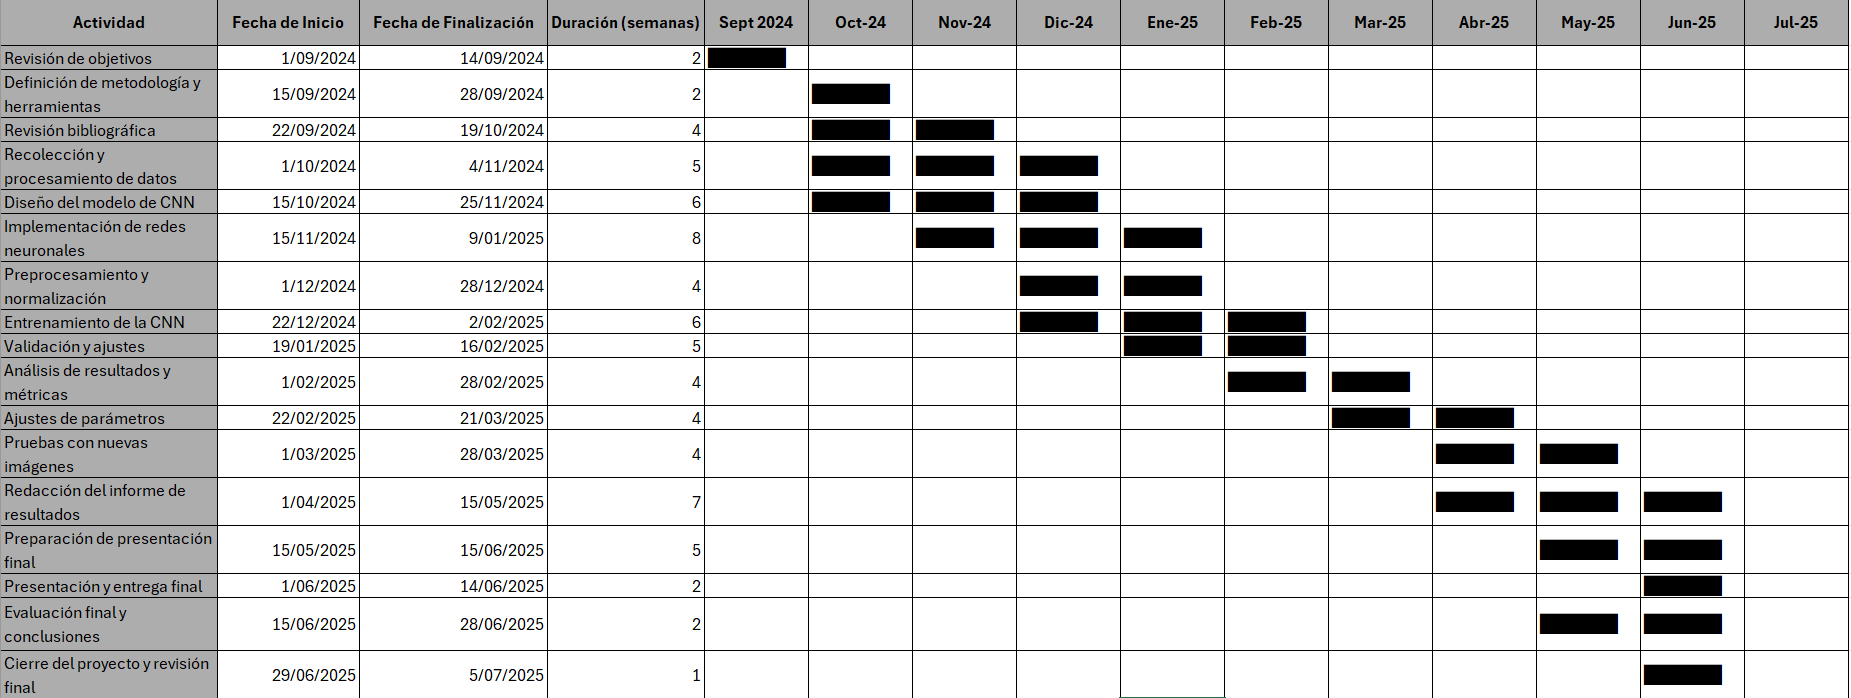
\includegraphics[width=1.50\textwidth]{3/figures/gant.png}
			\caption[Cronograma de actividades]{Cronograma de actividades.\\
				Fuente: Elaboración propia.}
			\label{3:fig8}
		\end{center}
	\end{figure}
	
\end{landscape}
%%%%%%%%%%%%%%%%%%%%%%%%%%%%%%%%%%%%%%%%

%%%%%%%%%%%%%%%%%%%%%%%%%%%%%%%



La Tabla \ref{tab:presupuesto} detalla los gastos relacionados con la investigación, incluyendo la compra de herramientas como una computadora portátil antes del inicio del proyecto, así como los costos asociados a actividades generales y al proceso de redacción y presentación pública de la tesis.

\begin{table}[h!]
	\caption{Presupuesto}
	\label{tab:presupuesto}
	\centering
	\small
	\begin{tabular}{p{6cm}rrr}
		\toprule
		\textbf{Concepto} & \textbf{Horas empleadas} & \textbf{Gasto (en soles)} & \textbf{Total} \\
		\midrule
		\multicolumn{4}{l}{\textbf{Activos físicos}} \\
		Portátil Lenovo Ideapad S340-15IIL Core i7 de 10ma GEN & -- & S/.5,700.00 & S/.5,700.00 \\
		\midrule
		\multicolumn{4}{l}{\textbf{Honorarios por el proceso de elaboración y defensa pública de la tesis}} \\
		Tasa de registro para el tema de investigación & -- & S/.800.00 & S/.800.00 \\
		Apartado del tema de tesis & -- & S/.2,700.00 & S/.2,700.00 \\
		Honorarios de defensa & -- & S/.1,500.00 & S/.1,500.00 \\
		\midrule
		\multicolumn{4}{l}{\textbf{Personal o equipo humano}} \\
		Progreso de tesis & 1000 & Inconmensurable & -- \\
		\midrule
		\multicolumn{4}{l}{\textbf{Gastos operativos}} \\
		Conexión a internet y servicio de electricidad (durante 8 meses) & 200 & S/.50.00 & S/.1000.00 \\
		\midrule
		\textbf{Python} & 50 & - & - \\
		\midrule
		\textbf{Suma total} & 1250 & -- & S/.11,700.00 \\
		\bottomrule
	\end{tabular}
	\begin{flushleft}
		\small Fuente: Elaboración propia.
	\end{flushleft}
\end{table}




